\section{Конструкторская часть}

В данном разделе будут представлена IDEF0 диаграмма разрабатываемой рекомендательной системы, а также будет рассмотрен и подробно описан каждый этап разработки, приведена схема, разрабатываемой рекомендательной системы, а также описан метод тестирования модели нечеткой кластеризации.

\subsection{Декомпозиция разрабатываемой рекомендательной системы}

Разрабатываемая рекомендательная система состоит из этапов.

\begin{itemize}
	\item предобработка входных данных;
	\item векторизация предобработанных данных;
	\item понижение размерности полученной матрицы;
	\item разделение новостей на кластеры;
	\item рекомендация новостей на основе данных, выделенных в кластеры.
\end{itemize}

Ниже представлена IDEF0-диаграмма разрабатываемого метода на рисунке \ref{idef0_big}.

\begin{figure}[H]
	\centering
	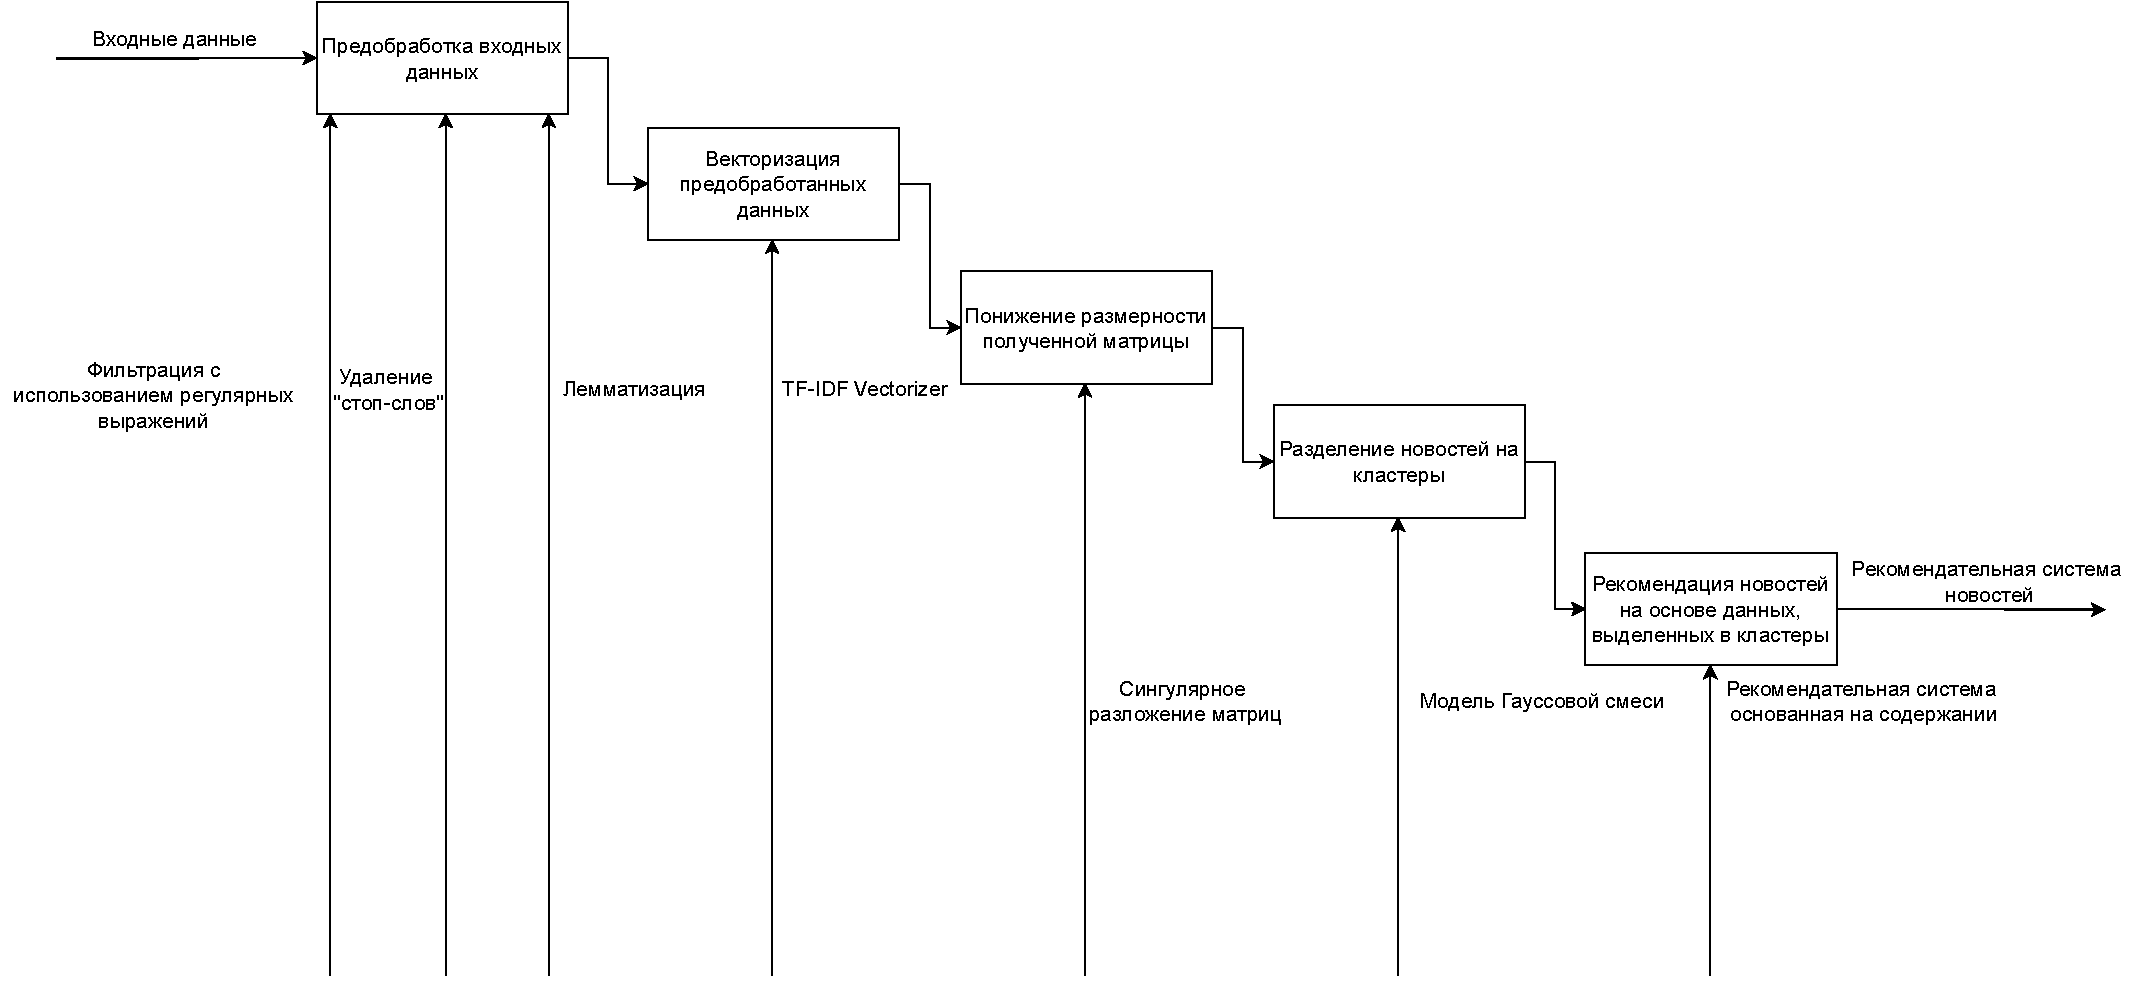
\includegraphics[width=\textwidth]{img/idef0_big.pdf}
	\caption{IDEF0-диаграмма}
	\label{idef0_big}
\end{figure}  

\subsection{Предобработка входных данных}

Данный этап предназначен для подготовки к дальнейшему обучению входных данных. На вход поступают структуры из json-файла, которые содержат информацию о новостях. Пример входных данных приведен в таблице \ref{input_data}

\begin{table}[H]
	\caption{Пример входных данных.}
	\label{input_data}
	\begin{center}
		\begin{tabularx}{1\textwidth}{ 
				| >{\centering\arraybackslash}X 
				| >{\centering\arraybackslash}X 
				| >{\centering\arraybackslash}X
				| >{\centering\arraybackslash}X 
				| >{\centering\arraybackslash}X | }
			\hline
			ID & Заголовок & Абстрактное описание & Новость & Дата публикации \\ 
			\hline
			N45436 & Walmart Slashes Prices on Last-Generation iPads & Apple's new iPad releases bring big deals on last year's models... &  This year, Walmart’s not waiting until to offer steep deals on tech. Right now, you can save big on since new models for 2019... & 10/29/2019 \\ 
			\hline
			N23144	& 50 Worst Habits For Belly Fat & These seemingly harmless habits are holding you back and keeping you from shedding that unwanted belly fat for good. & When you first start dieting and exercising, the pounds seem to melt off. But, we all hit that stagnant point where the last few pounds of belly fat just don’t want to leave... & 5/7/2019 \\ 
			\hline
		\end{tabularx}
	\end{center}
\end{table}

Для того, чтобы корректно произвести векторизацию и последующее обучение модели, данные следует предобработать следующим образом:

\begin{itemize}
	\item объединить столбцы с заголовком, абстрактным описанием и самой новостью;
	\item удалить все символы, кроме кириллических;
	\item удалить все "стоп-слова";
	\item провести лемматизацию.
\end{itemize}

После выполнения данного этапа будет получен массив предложений в которых содержится только необходимая для обучения информация, а все данные не несущие смысловую нагрузку удалены.

\subsection{Векторизация предобработанных данных}

Для векторизации полученных данных используется терм-документная частота (TF-IDF). Вычисление TF-IDF состоит из трех этапов

\begin{itemize}
	\item вычисление TF;
	\item вычисление IDF;
	\item Произведение TF и IDF и получение TF-IDF
\end{itemize}

TF (term frequency) позволяет оценить важность терма в отдельно взятом документе. TF вычисляется по формуле \ref{tf_des_formula}

\begin{equation}
\label{tf_des_formula}
TF(w, d) = \frac{n_w}{\sum_{i}n_i},
\end{equation}

где $n_w$ --- количество вхождений терма $w$ в документ $d$, $\sum_{i}n_i$ --- количество слов в документе.

Инверсная документная частота (Inverse Document Frequency (IDF)) необходима для уменьшения веса широко употребляемых слов. Вычисляется по формуле \ref{idf_des_formula}.

\begin{equation}
\label{idf_des_formula}
IDF(w_i, D) = \log{(\frac{|D|}{|D_i|})},
\end{equation}

где $|D|$ --- это общее количество документов, а $|D_i|$ --- это число документов, где $w_i$ встретилось хотя бы раз.

Получаем что TF-IDF вычисляется по формуле \ref{tf_idf_des_formula}

\begin{equation}
\label{tf_idf_des_formula}
TF-IDF(w_i, D) = TF(w, d) * IDF(w_id, D)
\end{equation}

Векторизация подобным образом очень эффективна для последующей задачи кластеризации, так как значимые термы, встречающиеся в пределах одного документа, но редко употребляемые во всем корпусе, имеют наибольший вес.

Результатом выполнения данного этапа является матрица, строки которой --- это документ (новость), а столбцы --- это все термы документов (новостей). В каждой ячейке хранятся TF-IDF для конкретного терма. Так как корпус состоит из большого количества уникальных слов, то матрица получается разреженная, а также слишком большого размера.

\subsection{Понижение размерности матрицы признаков}

На данном этапе производится сингулярное разложение, полученной на предыдущем шаге матрицы признаков. Данное действие обусловлено тем, что вычислительные мощности моего оборудования не позволяют обрабатывать таблицу подобного размера при проведении кластеризации. Также это сделано для увеличения скорости работы алгоритма нечеткой кластеризации, что немаловажно.


\subsection{Разделение новостей на кластеры}

После понижения размерности выполняется этап нечеткой кластеризации новостей из полученной матрицы. В качестве алгоритма нечеткой кластеризации используется модель Гауссовой смеси (Gaussian Mixture Model (GMM)), алгоритм работы которого приведен ниже.

В данном алгоритме каждый кластер представляется параметрическим распределением, а весь набор данных моделируется смесью этих распределений, следовательно для Гауссовой смеси получаем формулу \ref{gauss_formula}

\begin{equation}
\label{gauss_formula}
P({\bf x}\vert \Theta)=\sum_{i=1}^K \alpha_i p_i({\bf x}\vert \theta_i),
\end{equation}

где параметры $\Theta = (\alpha_1,...,\alpha_K, \theta_1,...,\theta_K)$ такие что $\sum_{i=1}^{K}\alpha_i = 1$ и каждое $p_i$ является функцией плотности Гаусса параметризованной по $\theta_i$. Другими словами, мы предполагаем, что у нас есть $K$ плотностей компонентов, смешанных вместе с $K$ коэффициентами смешения $\alpha_i$.

Пусть ${\cal X} = (x_1,...,x_m)$ --- это набор точек данных. Требуется найти такое $\Theta$, чтобы $p({\cal X}\vert\Theta)$ было максимальным. Подобная задача известна как оценка максимального правдоподобия для $\Theta$. Для оценки $\Theta$ обычно вводят логарифмическую функцию правдоподобия, определяемая по формуле \ref{L_formula}.

\begin{equation}
\label{L_formula}
{\cal L}(\Theta)={\rm log} P({\cal X}\vert \Theta)={\rm log} \prod_{i=1}^m P({\bf x}_i \vert \Theta) =\sum_{i=1}^m {\rm log} \left( \sum_{j=1}^K \alpha_j p_j({\bf x}_i\vert \theta_j)\right)
\end{equation}

Подобную функцию трудно оптимизировать, поскольку она содержит логарифм суммы. Для упрощения выражение правдоподобия, пусть $y_i\epsilon{1,…,K}$ обозначает, из какого Гауссиана $x_i$, и ${\cal Y}=(y1,...,ym)$. Если мы знаем значение ${\cal Y}$, получаем формулу \ref{L_final_formula}.

\begin{equation}
\label{L_final_formula}
\begin{matrix}
{\cal L}(\Theta)={\rm log} P({\cal X}, {\cal Y}\vert \Theta)={\rm log} \prod_{i=1}^m P({\bf x}_i, y_i\vert \Theta)=\\
=\sum_{i=1}^m{\rm log} P({\bf x}_i\vert y_i)P(y_i)=\sum_{i=1}^m{\rm log}( \alpha_{y_i} p_{y_i}({\bf x}_i \vert \theta_{y_i}))
\end{matrix}
\end{equation}

которая впоследствии оптимизируется с помощью различных методов, самым популярным из которых является алгоритм максимизации ожидания.

Исходя из названия становится ясно, что алгоритм состоит из двух частей, а именно вычисления ожидания (E), которое приведено в формулах \ref{Expectation_formula}, и вычисления максимизации (M), которое приведено в формулах \ref{Maximization_mu_formula}, \ref{Maximization_cov_formula} и \ref{Maximization_pi_formula}. Также используются вспомогательные формулы такие как \ref{Expectation_N_formula} и \ref{Expectation_normal_formula}.

\begin{equation}
\label{Expectation_normal_formula}
f(x; \mu, \sum) = \frac{1}{\sqrt{(2\pi) ^d * \det(\sum)}} * e^(\frac{-1}{2}*((x - \mu)^T * inv(\sum)*(x - \mu))),
\end{equation}

где $d$ --- длина вектора $x$, $x$ это выходной вектор, $\mu$ вектор средних, а $\sum$ это матрица ковариаций.

\begin{equation}
\label{Expectation_formula}
r_{n,k} = \frac{\pi_kN(x_n|\mu_k, \sum_k)}{\sum_j\pi_jN(x_n|\mu_j, \sum_j)},
\end{equation}

где $\pi_k$ и $pi_j$ --- это отношения количества элементов в кластере $k$ и $j$ соответственно ко всем элементам данных, $x_n$ это входной вектор данных, $\mu_k$ и $\mu_j$ это вектор средних для столбцов $k$ и $j$, вычисляемый по формуле \ref{Expectation_normal_formula}, а $\sum_k$ и $\sum_j$ это матрица ковариаций элементов в кластерах $k$ и $j$.

\begin{equation}
\label{Expectation_N_formula}
N = \sum_{k}r_{n,k}
\end{equation}

По формуле ожидания видно, что мы получаем матрицу в которой строки --- это каждый элемент данных, а столбец представляет кластер, следовательно каждый элемент данной матрицы это вероятность принадлежности элемента данных к столбцу. После того как алгоритм сойдется, данные из этой матрицы будут использованы в качестве предсказания точки кластера. Также на данном шаге вычисляется $N$ по формуле \ref{Expectation_N_formula}, которое представляет из себя список сумм столбцов матрицы $r_{n,k}$.

Схема алгоритма шага ожидания (E) приведена на рисунке \ref{E-step}.

\begin{figure}[H]
	\centering
	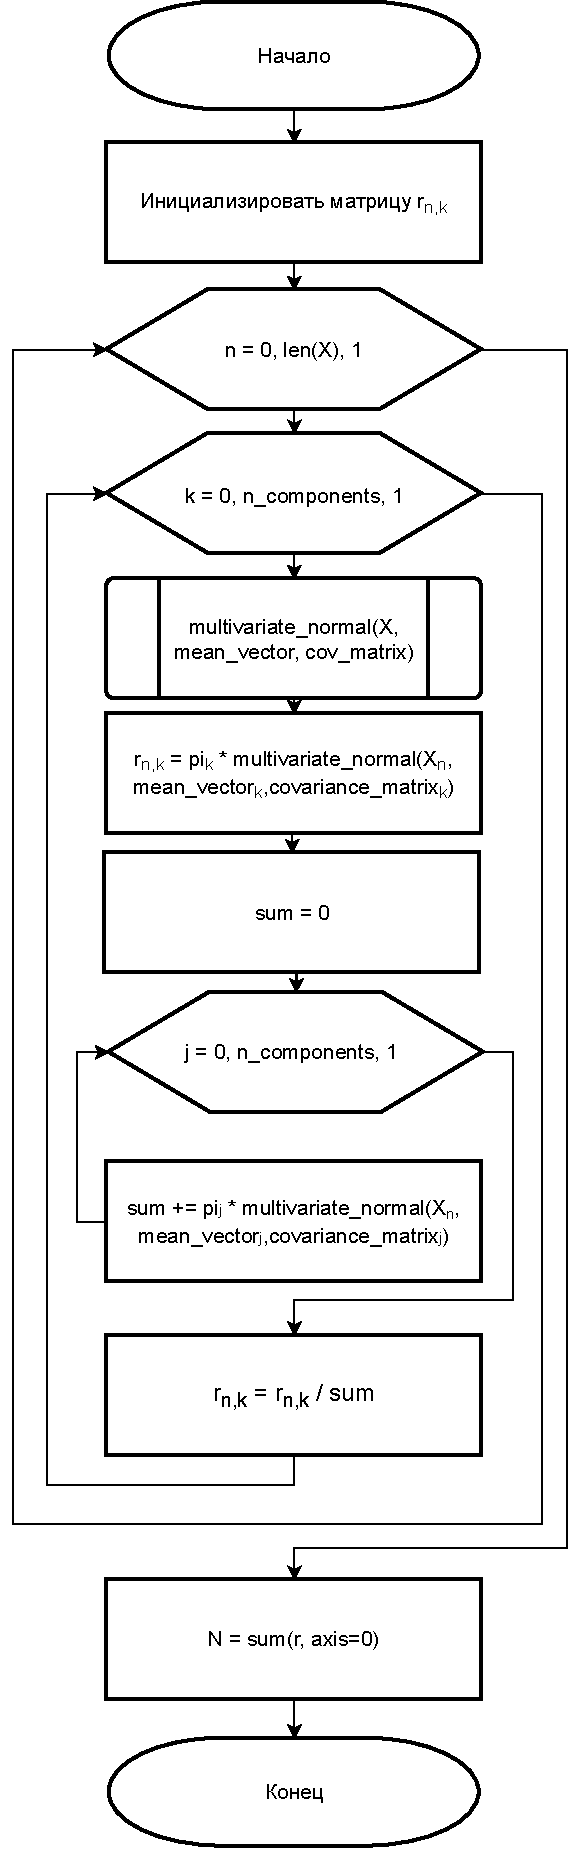
\includegraphics[scale=0.8]{img/E-step.pdf}
	\caption{Схема алгоритма шага ожидания}
	\label{E-step}
\end{figure}

Вычисления максимизации (M), приведено в формулах \ref{Maximization_mu_formula}, \ref{Maximization_cov_formula} и \ref{Maximization_pi_formula}.

\begin{equation}
\label{Maximization_mu_formula}
\mu_k = \frac{1}{N_k}\sum_{n=1}^{N}r_{n,k}x_n,
\end{equation}

\begin{equation}
\label{Maximization_cov_formula}
\sum_k = \frac{1}{N_k}\sum_{n=1}^{N}r_{n,k}(x_n - \mu_k)(x_n - \mu_k)^T,
\end{equation}

\begin{equation}
\label{Maximization_pi_formula}
\pi_k = \frac{N_k}{N},
\end{equation}

В формуле \ref{Maximization_mu_formula} вычисляется новый вектор средних для каждого столбца, в формуле \ref{Maximization_cov_formula} происходит обновление матрицы ковариаций для каждого столбца, а в формуле \ref{Maximization_pi_formula} обновляется список отношений количества элементов в кластере ко всем элементам данных.

Схема алгоритма шага максимизации (M) приведена на рисунке \ref{M-step}.

\begin{figure}[H]
	\centering
	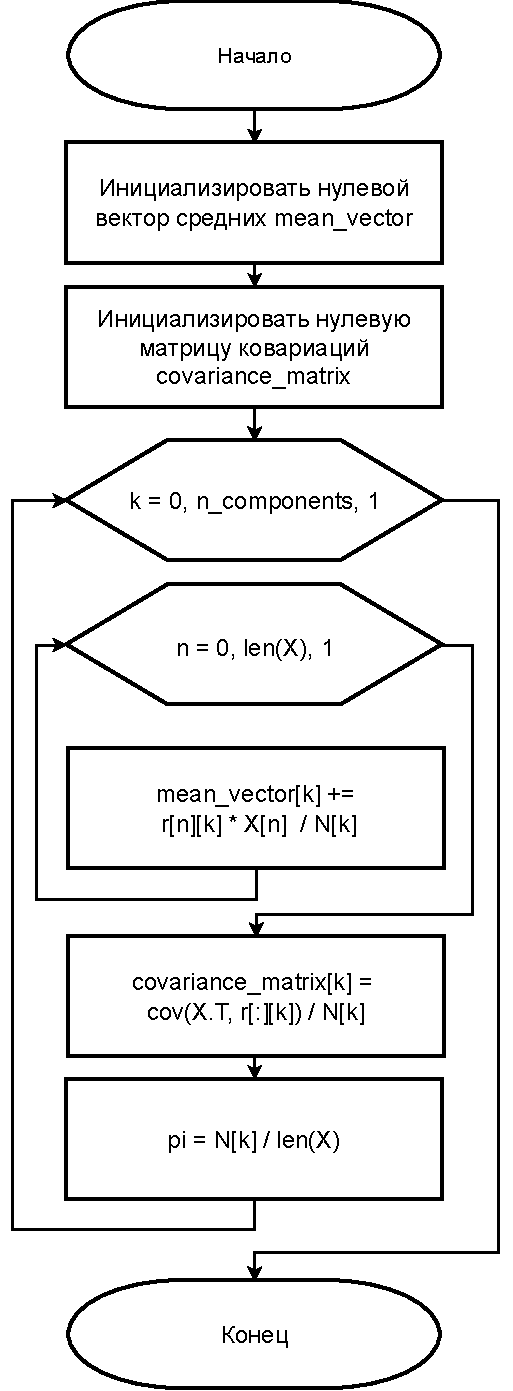
\includegraphics[scale=1]{img/M-step.pdf}
	\caption{Схема алгоритма шага максимизации}
	\label{M-step}
\end{figure}

Схема алгоритма метода максимизации ожидания для модели Гауссовой смеси представлена на рисунке \ref{EM}

\begin{figure}[H]
	\centering
	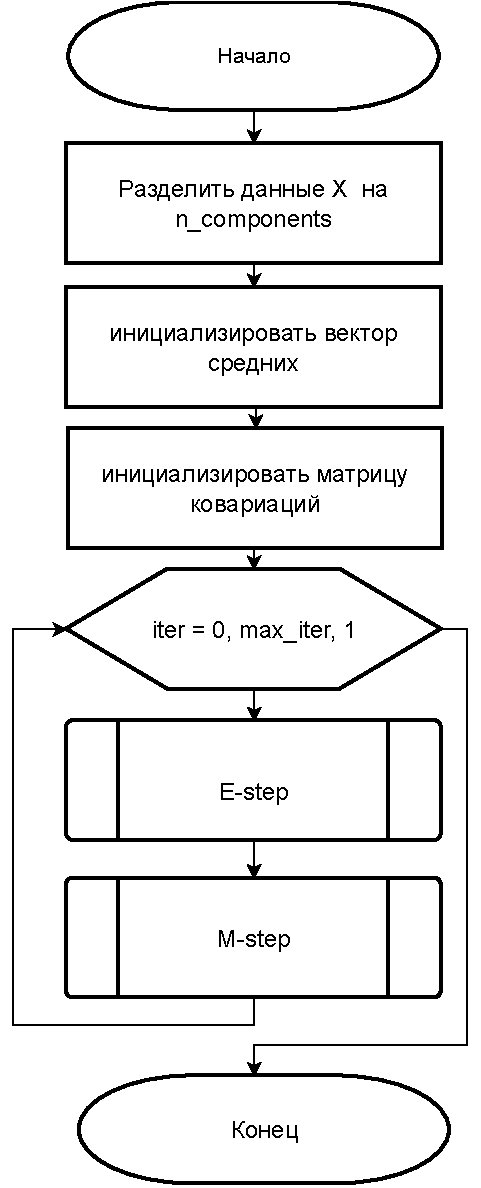
\includegraphics[scale=1]{img/EM.pdf}
	\caption{Схема алгоритма метода максимизации ожидания для модели Гауссовой смеси}
	\label{EM}
\end{figure}

\subsection{Рекомендация новостей на основе данных, выделенных в кластеры}

Заключительным этапом разработки приложения, является создание рекомендательной системы новостей на основе данных, полученных после проведения нечеткой кластеризации, а именно предоставление пользователю набора новостей из того же кластера, что и выбранная им новость и кластеров, центры которых наиболее близки к текущему. Результатом данного этапа является рекомендательная ситема, предоставляющая пользователю рекомендации новостей на основе его персональных предпочтений.

\subsubsection{Принцип работы рекомендательной системы}

Принцип работы рекомендательной системы приведен на схеме алгоритма, изображенной на рисунке \ref{RecsDiag}.

\begin{figure}[H]
	\centering
	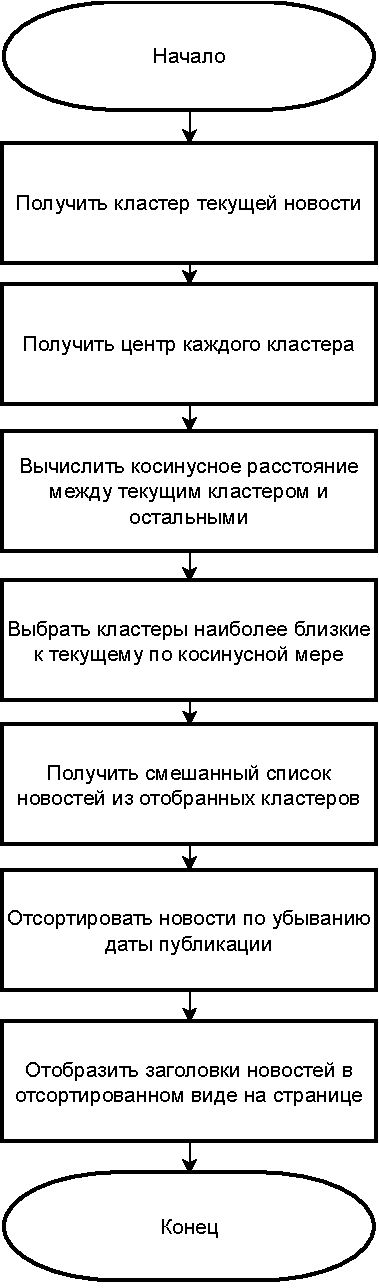
\includegraphics[scale=1]{img/RecsDiag.pdf}
	\caption{Схема рекомендательной системы на основе контента}
	\label{RecsDiag}
\end{figure}

Для того, чтобы выполнить корректную рекомендацию требуется предварительно провести действия, описанные выше. Следовательно перед самой рекомендацией новости требовалось предобработать для корректной работы алгоритма, а также провести понижение размерности для ускорения скорости работы, пожертвовав незначительным количество информации

\subsection{Тестирование обученной модели}

Поскольку у нас нет априорных данных о принадлежности новостей к категориям, требуется выбрать такой критерий оценки, который позволит оценить насколько объект похож на свой кластер по сравнению с другими кластерами. Данную задачу наилучшим образом решает метод оценки качества под названием Силуэт (Silhouette). Метод силуэтов --- способ изучения разделительного расстояния между результирующими кластерами наблюдений, данная мера имеет диапазон [-1, 1]. Коэффициенты силуэта около +1 указывают на то, что образец находится далеко от соседних кластеров. Значение, близкое к нулю указывает, что выборка находится на границе принятия решения между двумя соседними кластерами или очень близко к ней, а отрицательные значения указывают на то, что эти выборки могли быть назначены неправильному кластеру.

Оценка для всей кластерной структуры приведена в формуле \ref{Sil_C_formula}

\begin{equation}
\label{Sil_C_formula}
Sil(C) = \frac{1}{N}\sum_{c_k\epsilon C}\sum_{x_i\epsilon c_k}\frac{b(x_i, c_k) - a(x_i, c_k)}{max\{a(x_i, c_k), b(x_i, c_k)\}},
\end{equation}

где $a(x_i, c_k) = \frac{1}{|c_k|}\sum_{x_j\epsilon c_k}||x_i - x_j||$ --- среднее расстояние от $x_i \epsilon c_k$ до других объектов из кластера $c_k$ (компактность),

$b(x_i, c_k) = min_{c_l\epsilon C}\{\frac{1}{|c_l|}\sum_{x_j \epsilon c_l}||x_i - x_j||\}$ --- среднее расстояние от $x_i \epsilon c_k$ до объектов из другого кластера $c_l : k \neq l$ (отделимость).

По формуле \ref{Sil_C_formula} можно заметить, что

$-1 \leqslant Sil(C) \leqslant 1.$

И чем ближе данная оценка к 1, тем лучше.

Более того для тестирования реализованной модели нечеткой кластеризации и ее сравнения с моделью из библиотеки scikit-learn, потребуется оценка способная дать более точный результат называемая V-мерой, так как она использует информацию о том к каким кластерам принадлежат данные.

V-мера представляет из себя гармоническое среднее оценки однородности и полноты. Вычисление V-меры представлено в формуле \ref{v_measure}

\begin{equation}
\label{V_measure}
V-measure = 2 * \frac{h * c}{h + c},
\end{equation}

где $h$ --- это однородность, представленная в формуле \ref{Homogenity}, а $c$ --- полнота и представлена она в формуле \ref{Completeness}.

Однородность измеряет, насколько образцы в кластере похожи и измеряется с помощью энтропии Шеннона. Вычисление однородности приведено в формуле \ref{Homogenity}, энтропия Шеннона для образцов с назначенным кластером $C$ в кластере $K$ приведена в формуле \ref{Shannon}.

\begin{equation}
\label{Shannon}
H(C|K) = -\sum\frac{n_{ck}}{N}\log(\frac{n_{ck}}{n_k}),
\end{equation}

где $n_{ck}$ --- это количество образцов из кластера $c$ в кластере $k$, $n_k$ это общее количество образцов в кластере $c$, а $N$ размер набора данных.

\begin{equation}
\label{Homogenity}
h = 1 - \frac{H(C|K)}{H(C)}
\end{equation}

Как можно заметить, если все образцы в кластере $k$ имеют одинаковый назначенный кластер $c$, то однородность равна 1.

Полнота же измеряет, сколько похожих образцов объединяется алгоритмом кластеризации. Формула вычисления полноты приведена в формуле \ref{Completeness}.

\begin{equation}
\label{Completeness}
c = 1 - \frac{H(K|C)}{H(K)},
\end{equation}

где $H(K|C)$ отражает энтропию отношения образцов из кластера $c$ в кластере $k$ к общему количеству образцов $c$.

Если все образцы с назначенным кластером $c$ назначены одному кластеру $k$, то полнота равна 1.


\subsection{Выводы из конструкторского раздела}

В данном разделе была представлена IDEF0 диаграмма разрабатываемой рекомендательной системы, далее были рассмотрены все этапы разработки, а именно:
\begin{itemize}
	\item этап предобработки входных данных;
	\item этап векторизации предобработанных данных;
	\item этап понижения размерности матрицы признаков;
	\item этап разделения новостей на кластеры;
	\item этап рекомендации новостей.
\end{itemize}

Также была приведена схема алгоритма метода максимизации ожидания для модели Гауссовой смеси, а также схема алгоритма как шага ожидания, так и шага максимизации данного алгоритма. Приведена схема рекомендательной системы и описан метод тестирования обученной модели с использованием разных методов оценки.

\pagebreak